% **************************************************************************************************************
%
%  Copyright 2020-2026 Robert Bosch GmbH
%
%  Licensed under the Apache License, Version 2.0 (the "License");
%  you may not use this file except in compliance with the License.
%  You may obtain a copy of the License at
%
%      http://www.apache.org/licenses/LICENSE-2.0
%
%  Unless required by applicable law or agreed to in writing, software
%  distributed under the License is distributed on an "AS IS" BASIS,
%  WITHOUT WARRANTIES OR CONDITIONS OF ANY KIND, either express or implied.
%  See the License for the specific language governing permissions and
%  limitations under the License.
%
% **************************************************************************************************************

\section{Description}

\subsection{Introduction}

ProcessHub is a process lifecycle management system designed for distributed test automation environments.
It provides a centralized hub for starting, stopping, monitoring, and coordinating processes across multiple
client panels. The system is built with clean architecture principles, ensuring testability, maintainability,
and extensibility.

\subsubsection{Key Features}

\begin{itemize}
   \item \textbf{Process Lifecycle Management}: Start, stop, and monitor processes with health checking
   \item \textbf{Multi-Client Coordination}: Multiple panels can share and coordinate process ownership
   \item \textbf{Restart Orchestration}: Coordinated restart protocol with acknowledgment from all affected clients
   \item \textbf{Pluggable Transport}: ZMQ, EventBus (RabbitMQ), or in-memory for testing
   \item \textbf{Platform Abstraction}: Windows and Unix process handling
   \item \textbf{Web Dashboard}: Real-time monitoring via browser (FastAPI-based)
   \item \textbf{Logging Integration}: Optional centralized logging (Fluentbit, Telegraf)
   \item \textbf{Fleet Orchestrator}: Coordinate multiple ProcessHub instances across PCs from a central point
\end{itemize}

\subsubsection{Design Philosophy}

ProcessHub follows several key design principles:

\begin{enumerate}
   \item \textbf{Separation of Concerns}: Core business logic is isolated from I/O, transport, and UI
   \item \textbf{Dependency Injection}: All external dependencies are injected, enabling easy testing
   \item \textbf{Protocol-Oriented}: Components communicate through well-defined protocols (interfaces)
   \item \textbf{Explicit State Machines}: Complex state transitions use explicit FSM patterns
   \item \textbf{Immutable Snapshots}: UI receives immutable copies of state, avoiding lock contention
\end{enumerate}

% ============================================================================
\subsection{Architecture Overview}
% ============================================================================

ProcessHub is organized into distinct layers, each with specific responsibilities:

\begin{figure}[h]
\centering
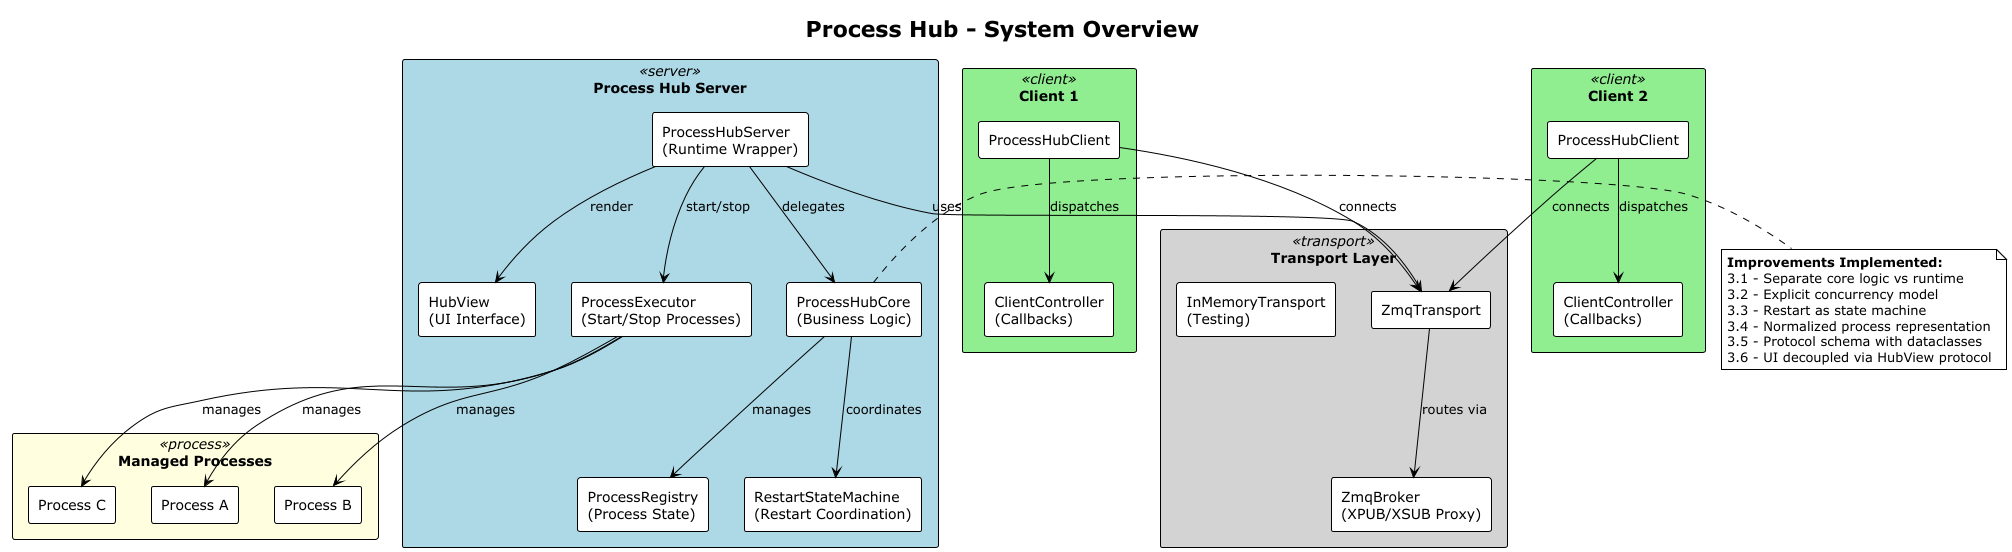
\includegraphics[width=0.95\textwidth]{../additional_docs/pictures/overview.png}
\caption{Process Hub System Overview}
\label{fig:overview}
\end{figure}

\subsubsection{Layer Responsibilities}

\begin{description}
   \item[Core Layer] Pure business logic without I/O dependencies. Contains the hub logic,
        process registry, restart state machine, and data models.

   \item[Transport Layer] Message passing abstraction. Provides ZMQ for local production,
        EventBus (RabbitMQ) for distributed environments, and in-memory transport for testing.
        All implement the same interface.

   \item[Runtime Layer] Server and client wiring. Thin wrappers that connect core logic
        to transport and UI. Contains the main event loops.

   \item[Process Layer] Process execution and platform-specific handling. Abstracts
        subprocess management for Windows and Unix platforms.

   \item[UI Layer] View implementations. Console TUI, null view for headless operation,
        and web dashboard for browser-based monitoring.

   \item[Config Layer] Configuration loading and validation. Supports JSON/YAML configs
        with schema validation.

   \item[Logging Layer] Optional integration with centralized logging servers like
        Fluentbit or Telegraf.

   \item[Fleet Layer] Optional overlay for multi-hub coordination. Contains the
        FleetOrchestrator (central coordinator), HubAgent (sidecar per hub),
        FleetClient (CI/CD API), HubRegistry (hub tracking), and FleetWebAPI
        (REST dashboard). Does not modify any other layer.
\end{description}

% ============================================================================
\subsection{Component Architecture}
% ============================================================================

The component diagram shows how packages relate to each other:

\begin{figure}[h]
\centering
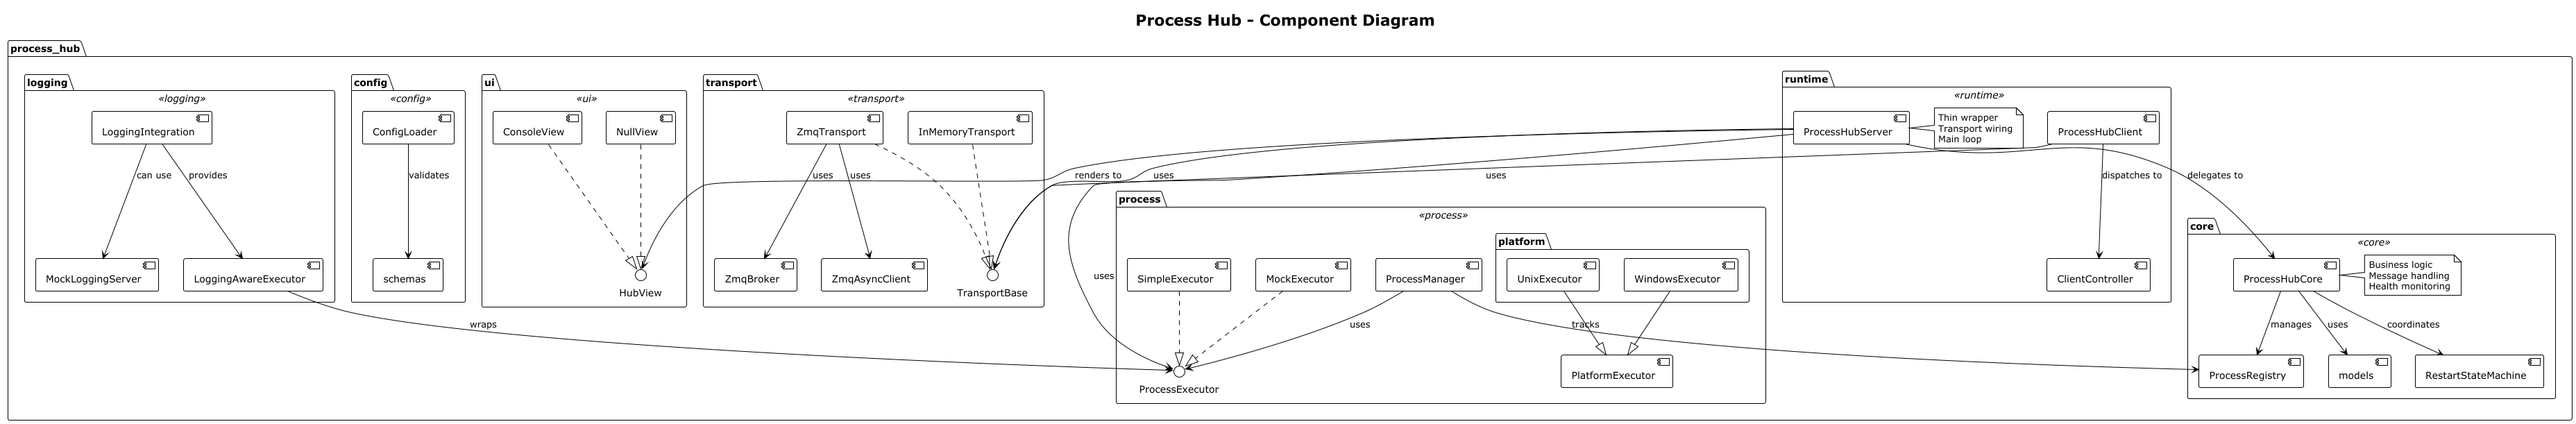
\includegraphics[width=0.95\textwidth]{../additional_docs/pictures/component.png}
\caption{Process Hub Component Diagram}
\label{fig:component}
\end{figure}

\subsubsection{ProcessHubCore}

The central business logic component implements improvement 3.1 (Separate core logic vs runtime):

\begin{itemize}
   \item Handles all message processing via \texttt{handle\_message()} method
   \item Manages process registry for tracking process state
   \item Coordinates restart state machine for multi-client restart
   \item Provides immutable state snapshots for UI rendering
   \item Has no direct knowledge of ZMQ, TUI, or file I/O
\end{itemize}

\begin{verbatim}
# ProcessHubCore is testable without I/O
core = ProcessHubCore(
    process_starter=mock_start,
    process_stopper=mock_stop,
    health_checker=mock_health,
)

# Handle message returns outgoing messages
outgoing = core.handle_message(incoming_msg)

# Get state snapshot (immutable, no locks needed)
snapshot = core.get_state_snapshot()
\end{verbatim}

\subsubsection{ProcessRegistry}

Thread-safe registry implementing improvement 3.4 (Normalized process representation):

\begin{itemize}
   \item Maintains process information: state, PID, requesters
   \item Supports multiple panels requesting the same process
   \item Provides atomic state transitions under single lock
   \item Returns immutable snapshots for concurrent access
\end{itemize}

\textbf{Process States:}

\begin{description}
   \item[REGISTERED] Process is known but not yet started
   \item[STARTING] Process start has been requested, waiting for confirmation
   \item[RUNNING] Process is confirmed running
   \item[STOPPING] Process stop has been requested
   \item[STOPPED] Process has exited normally
   \item[DEAD] Process was running but died unexpectedly
   \item[FAILED] Process failed to start
\end{description}

\subsubsection{RestartStateMachine}

Implements improvement 3.3 (Restart as explicit state machine):

\begin{figure}[h]
\centering
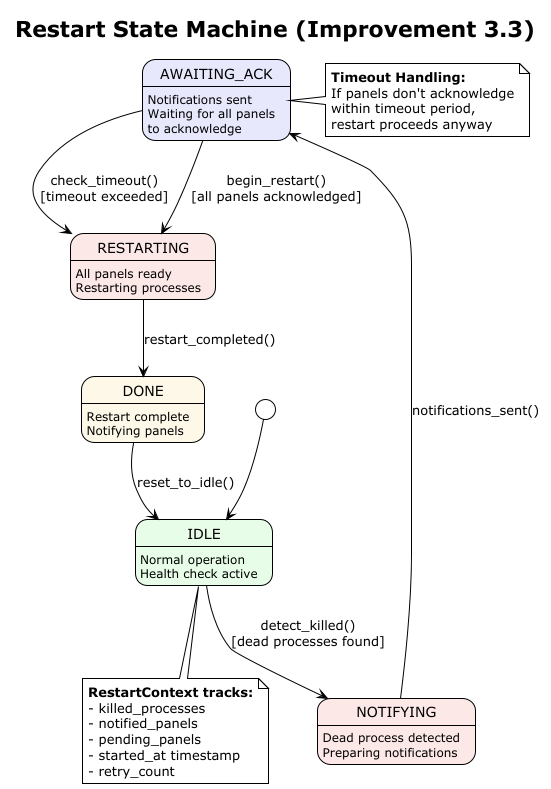
\includegraphics[width=0.8\textwidth]{../additional_docs/pictures/state_restart.png}
\caption{Restart State Machine}
\label{fig:restart_state}
\end{figure}

The state machine manages the complete restart coordination flow:

\begin{verbatim}
IDLE -> NOTIFYING -> AWAITING_ACK -> RESTARTING -> DONE -> IDLE
                           |              |
                        FAILED -----------+--------> IDLE
\end{verbatim}

\textbf{RestartContext} holds all restart-related data under a single lock:
\begin{itemize}
   \item \texttt{killed\_processes}: List of dead processes detected
   \item \texttt{notified\_panels}: All panels that were notified
   \item \texttt{pending\_panels}: Panels that haven't acknowledged yet
   \item \texttt{started\_at}: Timestamp for timeout detection
   \item \texttt{retry\_count}: Number of restart attempts
\end{itemize}

% ============================================================================
\subsection{Communication Patterns}
% ============================================================================

\subsubsection{Transport Abstraction}

All communication goes through the transport layer, which provides a unified interface:

\begin{verbatim}
class TransportBase(ABC):
    @abstractmethod
    def start(self) -> None: ...

    @abstractmethod
    def stop(self) -> None: ...

    @abstractmethod
    def send(self, topic: str, message: dict) -> None: ...

    @abstractmethod
    def subscribe(self, topic: str, callback: Callable) -> None: ...
\end{verbatim}

\subsubsection{ZMQ Transport}

Production transport using ZeroMQ PUB/SUB with XPUB/XSUB broker:

\begin{itemize}
   \item \textbf{XPUB/XSUB Broker}: Central message routing with subscription forwarding
   \item \textbf{Topic-based Filtering}: Messages routed by topic prefix
   \item \textbf{Async Client}: Background thread with event loop for non-blocking operation
   \item \textbf{Subscription Propagation}: Delay to ensure subscriptions reach broker
\end{itemize}

\begin{verbatim}
# Server with broker
server_transport = ZmqTransport(
    start_broker=True,
    xpub_port=5555,
    xsub_port=5556,
)

# Client connects to broker
client_transport = ZmqTransport(
    start_broker=False,
    xpub_port=5555,
    xsub_port=5556,
)
\end{verbatim}

\subsubsection{In-Memory Transport}

Testing transport for unit tests without network:

\begin{itemize}
   \item Direct message passing between server and clients
   \item Synchronous operation for predictable test behavior
   \item Full protocol compatibility with ZMQ transport
\end{itemize}

\subsubsection{EventBus Transport}

RabbitMQ-based transport using the EventBusClient library for enterprise message passing:

\begin{itemize}
   \item \textbf{RabbitMQ Backend}: Robust message broker with persistence and clustering
   \item \textbf{Topic Exchange}: Flexible routing with topic-based message filtering
   \item \textbf{Auto-reconnect}: Automatic reconnection on connection loss
   \item \textbf{JSON Serialization}: Human-readable message format
   \item \textbf{Client Events}: Event-based notifications for connection state changes
\end{itemize}

\textbf{Prerequisites:}

\begin{verbatim}
# 1. Install RabbitMQ (Docker recommended)
docker run -d -p 5672:5672 -p 15672:15672 rabbitmq:management

# 2. Install EventBusClient package
git clone https://github.com/test-fullautomation/python-rabbitmq-messagebus.git
cd python-rabbitmq-messagebus && pip install -e .
\end{verbatim}

\textbf{Server Configuration:}

\begin{verbatim}
from ProcessHub.transport.eventbus_transport import EventBusTransport

# Server transport
server_transport = EventBusTransport(
    host="localhost",
    port=5672,
    exchange_name="process_hub",
)
\end{verbatim}

\textbf{Client Configuration:}

\begin{verbatim}
# Client transport (same configuration)
client_transport = EventBusTransport(
    host="localhost",
    port=5672,
    exchange_name="process_hub",
)

# With config file
client_transport = EventBusTransport(config_path="eventbus_config.jsonp")
\end{verbatim}

\textbf{Client Events:}

The EventBus transport provides event notifications via the \texttt{ClientEvent} enum:

\begin{description}
   \item[CONNECTED] Client successfully connected to RabbitMQ
   \item[DISCONNECTED] Client disconnected from RabbitMQ
   \item[RECONNECTING] Client attempting to reconnect
   \item[ERROR] An error occurred during communication
\end{description}

\begin{verbatim}
from ProcessHub.transport.eventbus_transport import ClientEvent

def on_client_event(event: ClientEvent, data: dict):
    if event == ClientEvent.CONNECTED:
        print("Connected to RabbitMQ")
    elif event == ClientEvent.DISCONNECTED:
        print(f"Disconnected: {data.get('reason')}")

transport.register_event_handler(on_client_event)
\end{verbatim}

\textbf{EventBus Config File Format:}

\begin{verbatim}
{
    "host": "localhost",
    "port": 5672,
    "exchange_name": "process_hub",
    "exchange_handler": "TopicExchangeHandler",
    "serializer": "JsonSerializer",
    "auto_reconnect": true,
    "reconnect_delay": 5.0
}
\end{verbatim}

% ============================================================================
\subsection{Restart Coordination Protocol}
% ============================================================================

When a process dies unexpectedly, ProcessHub coordinates a restart across all affected clients:

\begin{figure}[h]
\centering
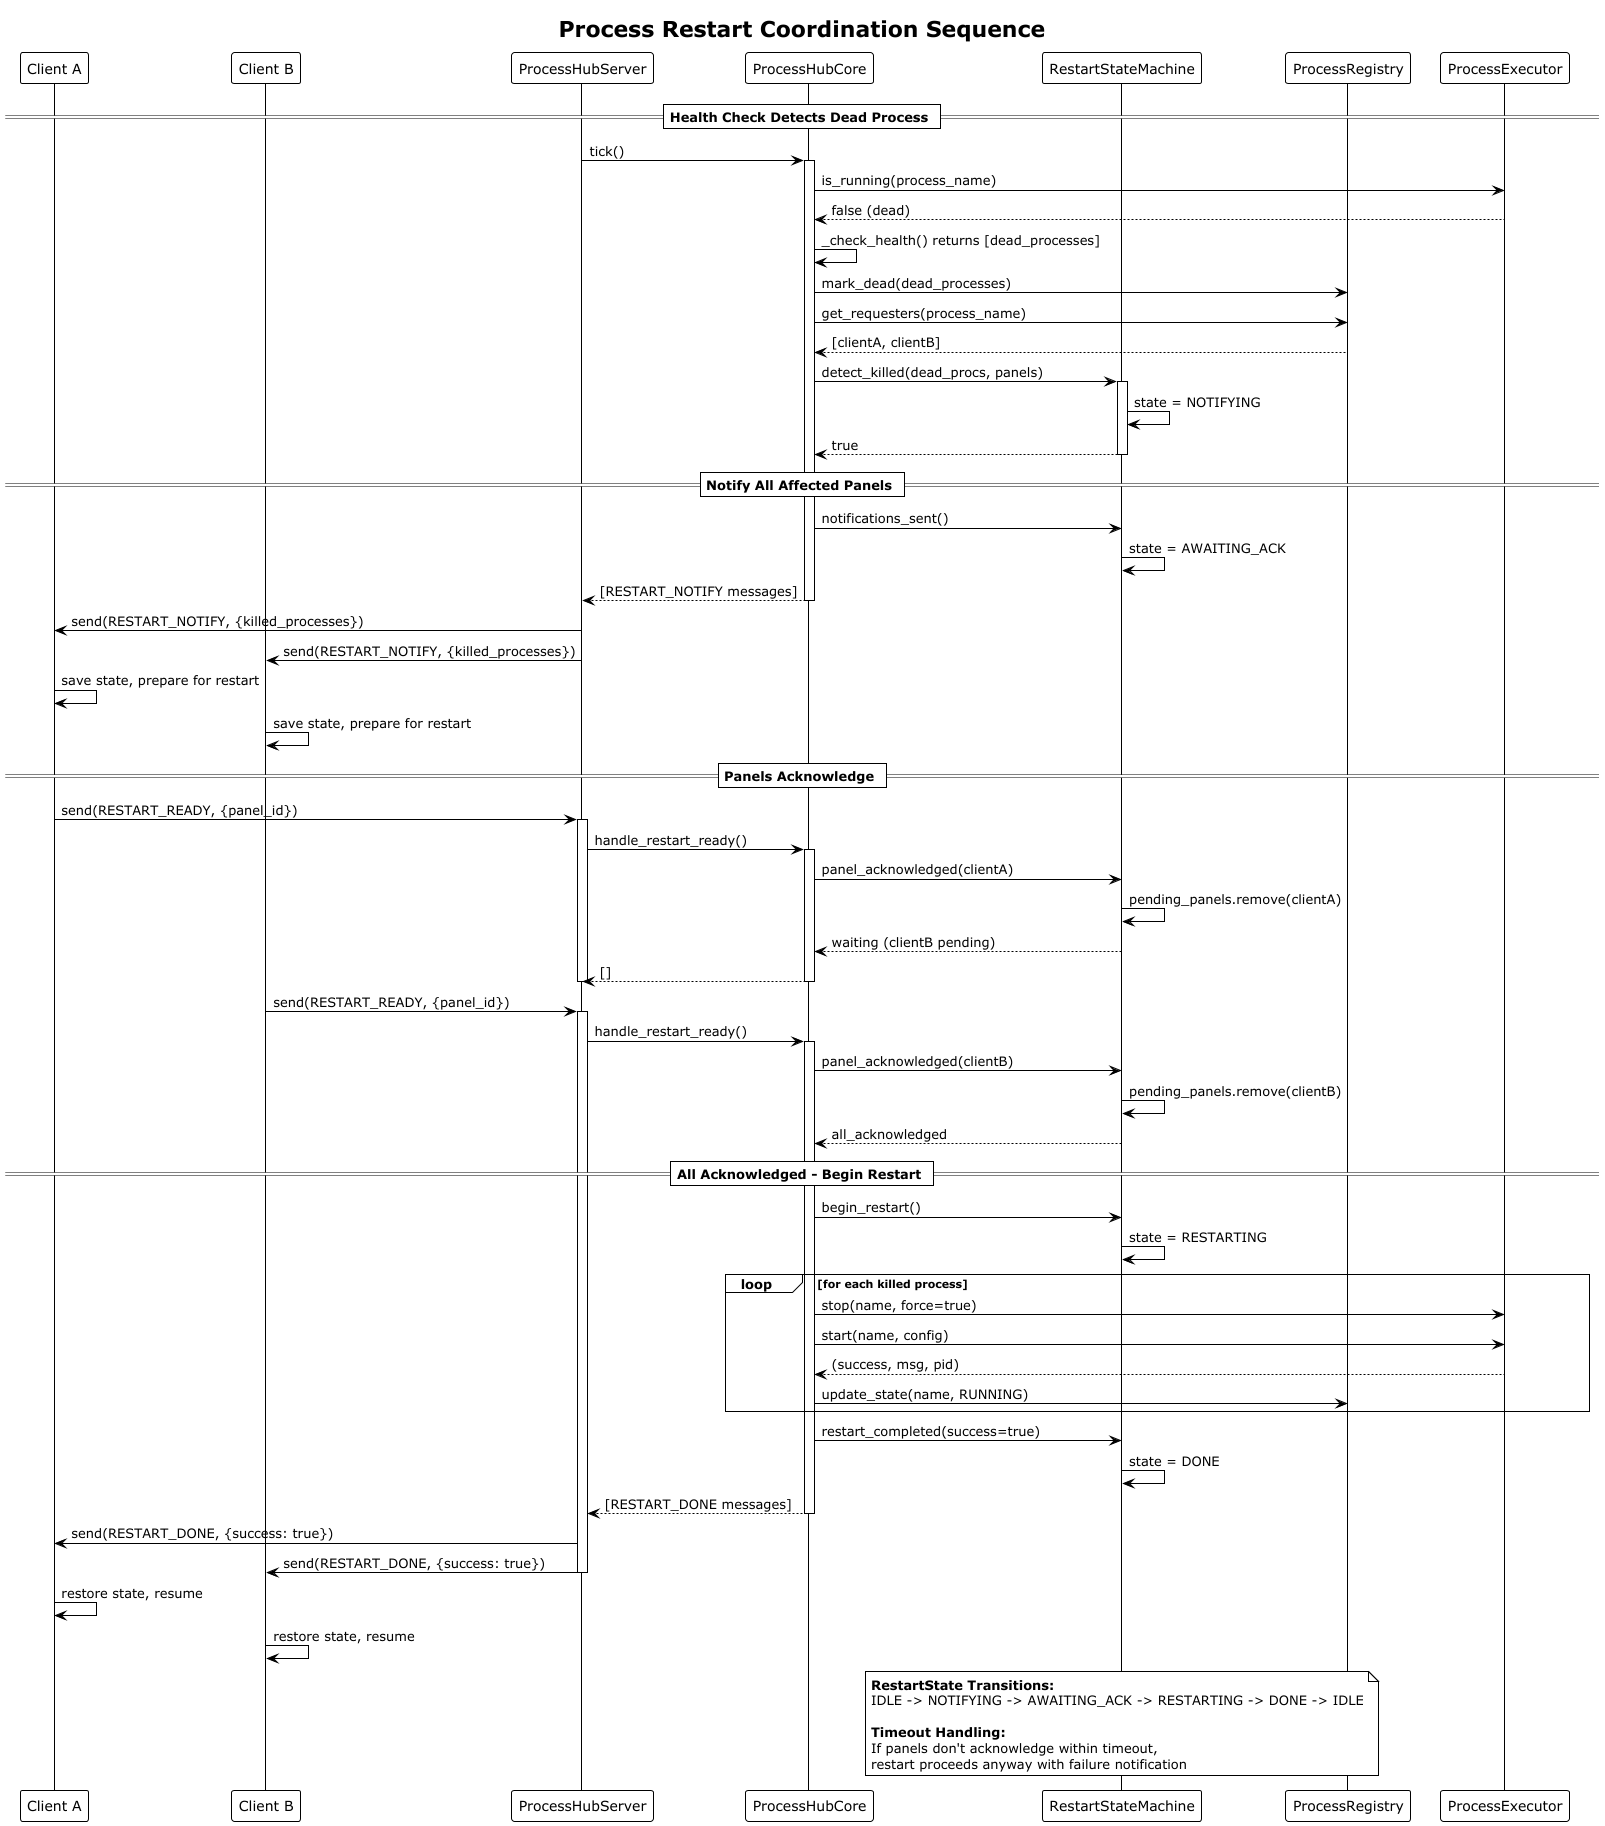
\includegraphics[width=0.95\textwidth]{../additional_docs/pictures/sequence_restart_flow.png}
\caption{Restart Coordination Sequence}
\label{fig:restart_sequence}
\end{figure}

\subsubsection{Protocol Flow}

\begin{enumerate}
   \item \textbf{Detection}: Health check detects dead process
   \item \textbf{Notification}: Server sends \texttt{ProcessRestartNotify} to all affected panels
   \item \textbf{Acknowledgment}: Each panel saves state and sends \texttt{ProcessRestartReady}
   \item \textbf{Restart}: Once all panels acknowledge (or timeout), server restarts processes
   \item \textbf{Completion}: Server sends \texttt{ProcessRestartDone} to all panels
   \item \textbf{Resume}: Panels restore state and resume operation
\end{enumerate}

\subsubsection{Timeout Handling}

If panels don't acknowledge within the configured timeout:

\begin{itemize}
   \item Restart proceeds anyway to avoid deadlock
   \item Non-responsive panels receive failure notification
   \item Timeout is configurable via \texttt{restart\_timeout} parameter
\end{itemize}

% ============================================================================
\subsection{Protocol Messages}
% ============================================================================

ProcessHub uses typed dataclass messages implementing improvement 3.5 (Protocol schema):

\subsubsection{Message Base}

All messages inherit from \texttt{MessageBase}:

\begin{verbatim}
@dataclass
class MessageBase:
    version: str = "1.0"
    timestamp: float = field(default_factory=time.time)
    request_id: Optional[str] = None
\end{verbatim}

\subsubsection{Connection Messages}

\begin{description}
   \item[RegisterConnectionRequest] Client registers with server
   \item[RegisterConnectionResponse] Server confirms registration
   \item[UnregisterConnectionRequest] Client disconnects
   \item[ConnectionInfoRequest] Client requests connection list
\end{description}

\subsubsection{Process Control Messages}

\begin{description}
   \item[ProcessStartRequest] Client requests process start
   \item[ProcessStartResponse] Server confirms start result
   \item[ProcessStopRequest] Client requests process stop
   \item[ProcessStopResponse] Server confirms stop result
\end{description}

\subsubsection{Restart Messages}

\begin{description}
   \item[ProcessRestartNotify] Server notifies panel of dead processes
   \item[ProcessRestartReady] Panel acknowledges ready for restart
   \item[ProcessRestartDone] Server notifies restart completion
\end{description}

% ============================================================================
\subsection{Web Dashboard}
% ============================================================================

ProcessHub includes an optional web-based dashboard built with FastAPI:

\begin{verbatim}
from ProcessHub.ui import WebView

view = WebView(host="0.0.0.0", port=2507)
server = ProcessHubServer(transport=transport, view=view)
server.run()

# Dashboard: http://localhost:2507
# API docs: http://localhost:2507/docs
\end{verbatim}

\subsubsection{Features}

\begin{itemize}
   \item \textbf{Real-time Dashboard}: Auto-refreshing status display
   \item \textbf{Connection Monitoring}: View all connected panels
   \item \textbf{Process Status}: Track process states and PIDs
   \item \textbf{Restart Visualization}: Monitor restart coordination progress
   \item \textbf{REST API}: Programmatic access to hub state
   \item \textbf{Auto-generated Docs}: Swagger UI at \texttt{/docs}, ReDoc at \texttt{/redoc}
\end{itemize}

\subsubsection{API Endpoints}

\begin{description}
   \item[GET /] Dashboard HTML page
   \item[GET /api/state] Complete hub state (connections, processes, restart)
   \item[GET /api/connections] List of connected panels
   \item[GET /api/processes] List of managed processes
   \item[GET /api/restart] Current restart coordination state
   \item[GET /api/health] Health check endpoint
\end{description}

% ============================================================================
\subsection{Logging Integration}
% ============================================================================

ProcessHub supports optional integration with centralized logging servers:

\begin{itemize}
   \item \textbf{Fluentbit}: Log aggregation and forwarding
   \item \textbf{Telegraf}: Metrics collection
   \item \textbf{Custom}: User-defined logging servers via protocol
\end{itemize}

\begin{verbatim}
from ProcessHub.logging import LoggingIntegration, LoggingServerType

logging = LoggingIntegration(
    server_type=LoggingServerType.FLUENTBIT,
    paths={
        "src_dir": "/path/to/fluentbit/config",
        "hot_dir": "/path/to/hot/reload",
        "ctrl_dir": "/path/to/control",
    },
    taf_path="/opt/taf",
)
logging.start()

# Get logging config for a process
config = logging.get_process_logging_config("my_process", {
    "central_log": True  # Enable for this process
})

# Enhance process args with logging
args = config.to_command_args(taf_path="/opt/taf")
\end{verbatim}

\subsubsection{LoggingAwareExecutor}

Wraps an executor to automatically add logging configuration:

\begin{verbatim}
from ProcessHub.logging import LoggingAwareExecutor

executor = LoggingAwareExecutor(
    executor=SimpleExecutor(),
    logging_integration=logging,
    process_configs=process_configs,
)
\end{verbatim}

% ============================================================================
\subsection{Fleet Orchestrator}
% ============================================================================

ProcessHub includes an optional \textbf{Fleet Orchestrator} for coordinating multiple ProcessHub
instances across different PCs from a central point. The fleet layer is a pure overlay -- it does
not modify the core, runtime, or transport modules.

\begin{verbatim}
                    +--------------------+
                    | FleetOrchestrator  |
                    |   (Central PC)     |
                    |   + HubRegistry    |
                    |   + FleetWebAPI    |
                    +---------+----------+
                              |
                 +------------+------------+
                 |  EventBus (RabbitMQ)    |
                 |  fleet.* routing keys   |
                 +----+-------+-------+---+
                      |       |       |
            +---------+  +----+----+  +----------+
            | Hub PC 1|  | Hub PC 2|  | Hub PC N |
            | HubAgent|  | HubAgent|  | HubAgent |
            | + Server|  | + Server|  | + Server |
            +---------+  +---------+  +----------+
\end{verbatim}

\subsubsection{Fleet Components}

\begin{description}
   \item[FleetOrchestrator] Central coordinator that discovers hubs via HubAnnounce messages,
        tracks hub health via heartbeat timeouts, routes commands from FleetClient to target hubs,
        and provides fleet-wide state snapshots. Runs a periodic \texttt{tick()} for health checking.

   \item[HubAgent] Lightweight sidecar that runs alongside each ProcessHubServer. Sends periodic
        heartbeats (HubAnnounce) and status reports (HubStatusReport) to the orchestrator. Handles
        incoming fleet commands (start\_process, stop\_process, reset, get\_status) by delegating
        to the local server's public API. Uses background daemon threads for heartbeat and status loops.

   \item[HubRegistry] Thread-safe registry of fleet hubs. Maintains mutable \_HubEntry objects
        internally, exposes immutable HubSnapshot and FleetStateSnapshot externally. Health state
        transitions: online (heartbeat within timeout/2) $\rightarrow$ degraded (within timeout)
        $\rightarrow$ offline (exceeded timeout).

   \item[FleetClient] High-level API for CI/CD pipelines, CLI tools, and scripts. Provides
        single-hub commands (start\_processes, stop\_processes, reset\_hub, get\_hub\_detail) and
        batch operations (start\_on\_all\_hubs, stop\_all\_processes, reset\_all\_hubs). Supports
        event callbacks via on\_hub\_online() and on\_hub\_offline().

   \item[FleetWebAPI] Optional REST API and HTML dashboard built with FastAPI. Provides endpoints
        for fleet status, hub listing, hub details, and command routing. HTML dashboard auto-refreshes
        every 5 seconds. Swagger documentation at \texttt{/docs}.
\end{description}

\subsubsection{Fleet Protocol Messages}

All fleet messages extend \texttt{MessageBase} for protocol versioning:

\begin{description}
   \item[HubAnnounce] Hub agent heartbeat and registration (hub\_id, hub\_name, host, capabilities)
   \item[HubRegistered] Orchestrator acknowledgement of new hub registration
   \item[HubDeregistered] Hub removal notification (graceful shutdown or timeout)
   \item[HubStatusReport] Periodic status from hub agent (process\_count, connection\_count, processes)
   \item[FleetCommand] Command from orchestrator to hub agent (command\_id, action, params)
   \item[FleetCommandResult] Result from hub agent back to orchestrator (success, message, data)
\end{description}

\subsubsection{Fleet Topics}

Fleet topics use the \texttt{FLEET\_} prefix to separate from local hub topics:

\begin{verbatim}
class FleetTopics(str, Enum):
    HUB_ANNOUNCE       = "FLEET_HUB_ANNOUNCE"
    HUB_REGISTERED     = "FLEET_HUB_REGISTERED"
    HUB_DEREGISTER     = "FLEET_HUB_DEREGISTER"
    HUB_STATUS_REPORT  = "FLEET_HUB_STATUS_REPORT"
    FLEET_COMMAND       = "FLEET_COMMAND"
    FLEET_COMMAND_RESULT = "FLEET_COMMAND_RESULT"
    HUB_ONLINE         = "FLEET_HUB_ONLINE"
    HUB_OFFLINE        = "FLEET_HUB_OFFLINE"
\end{verbatim}

\subsubsection{Fleet Quick Start}

\begin{verbatim}
from ProcessHub.fleet import FleetOrchestrator, HubAgent, FleetClient
from ProcessHub.transport.inmemory_transport import InMemoryTransport

# Central PC: Start orchestrator
fleet_transport = InMemoryTransport()
fleet_transport.start()

orchestrator = FleetOrchestrator(
    transport=fleet_transport, health_timeout=30.0
)
orchestrator.start()

# Hub PC: Attach agent to existing server
agent = HubAgent(
    server=my_server,
    transport=fleet_transport,
    hub_id="bench-1",
    hub_name="HIL Bench 1",
)
agent.start()

# CI/CD: Use FleetClient
client = FleetClient(
    transport=fleet_transport, orchestrator=orchestrator
)

# Check fleet health
snapshot = client.get_fleet_status()
print(f"Online: {snapshot.online_hubs}/{snapshot.total_hubs}")

# Start processes on a specific hub
client.start_processes("bench-1", ["ecu_simulator"])

# Batch operations across all online hubs
client.start_on_all_hubs(["data_logger"])
client.reset_all_hubs()
\end{verbatim}

\subsubsection{Fleet Web Dashboard}

\begin{verbatim}
from ProcessHub.fleet.web_api import FleetWebAPI

web = FleetWebAPI(
    orchestrator=orchestrator, host="0.0.0.0", port=2510
)
web.start()
# Dashboard: http://localhost:2510
# Swagger:   http://localhost:2510/docs
\end{verbatim}

\subsubsection{Fleet REST API Endpoints}

\begin{description}
   \item[GET /api/fleet/status] Fleet-wide status snapshot (total\_hubs, online\_hubs, hubs list)
   \item[GET /api/fleet/hubs] List all registered hubs
   \item[GET /api/fleet/hubs/\{hub\_id\}] Single hub details
   \item[POST /api/fleet/command] Send a command to a hub (hub\_id, action, params)
   \item[POST /api/fleet/hubs/\{hub\_id\}/start] Start processes on a hub
   \item[POST /api/fleet/hubs/\{hub\_id\}/stop] Stop processes on a hub
   \item[POST /api/fleet/hubs/\{hub\_id\}/reset] Reset a hub
   \item[GET /] HTML fleet monitoring dashboard (auto-refreshes every 5 seconds)
\end{description}

\subsubsection{Fleet Installation}

\begin{verbatim}
# Install with fleet support
pip install python-process-hub[fleet]

# Fleet web API requires FastAPI and uvicorn
pip install fastapi uvicorn
\end{verbatim}

% ============================================================================
\subsection{Installation}
% ============================================================================

\subsubsection{From PyPI}

\begin{verbatim}
# Basic installation
pip install python-process-hub

# With ZMQ support
pip install python-process-hub[zmq]

# With web dashboard
pip install python-process-hub[web]

# With fleet orchestrator
pip install python-process-hub[fleet]

# Development dependencies
pip install python-process-hub[dev]

# All optional dependencies
pip install python-process-hub[zmq,web,fleet,dev]
\end{verbatim}

\subsubsection{From Source}

\begin{verbatim}
# Clone repository
git clone https://github.com/test-fullautomation/python-process-hub.git
cd python-process-hub

# Install in development mode
python setup.py develop

# Or install normally
python setup.py install
\end{verbatim}

% ============================================================================
\subsection{Quick Start}
% ============================================================================

\subsubsection{Server Example}

\begin{verbatim}
import sys
from ProcessHub.runtime.server import ProcessHubServer
from ProcessHub.transport.zmq_transport import ZmqTransport
from ProcessHub.ui.console_view import ConsoleView
from ProcessHub.process.executor import SimpleExecutor

# Create transport with broker
transport = ZmqTransport(start_broker=True)

# Create view and executor
view = ConsoleView()
executor = SimpleExecutor()

# Define process configurations
process_config = {
    "system_manager": {
        "script": sys.executable,
        "args": ["-c", "import time; time.sleep(3600)"],
        "wait_time": 2.0,
    },
}

# Create and run server
server = ProcessHubServer(
    transport=transport,
    view=view,
    executor=executor,
    process_config=process_config,
)
server.run()  # Blocks until Ctrl+C
\end{verbatim}

\subsubsection{Client Example}

\begin{verbatim}
from ProcessHub.runtime.client import ProcessHubClient
from ProcessHub.transport.zmq_transport import ZmqTransport

# Connect to existing broker
transport = ZmqTransport(start_broker=False)
client = ProcessHubClient(transport=transport)
client.start()

# Register with server
client.register_connection(session_id="my_session")
client.wait_for_registration(timeout=10.0)

# Start processes
client.request_process_start(["system_manager"])

# Handle restart notifications via callbacks
def on_restart_notify(killed_processes):
    print(f"Processes died: {killed_processes}")
    # Save state, prepare for restart
    client.notify_restart_ready()

client.controller.connect("restart_notify", on_restart_notify)
\end{verbatim}

% ============================================================================
\subsection{Testing}
% ============================================================================

ProcessHub is designed for testability using the in-memory transport:

\begin{verbatim}
from ProcessHub.transport.inmemory_transport import InMemoryTransport
from ProcessHub.process.executor import MockExecutor

# Create in-memory transport (no ZMQ needed)
transport = InMemoryTransport()

# Create mock executor (no real processes)
executor = MockExecutor(process_configs)

# Test core logic without I/O
server = ProcessHubServer(
    transport=transport,
    executor=executor,
    view=NullView(),
)
\end{verbatim}

\subsubsection{Running Tests}

\begin{verbatim}
# Run all tests
pytest

# With coverage
pytest --cov=ProcessHub

# Specific test file
pytest tests/test_core.py -v
\end{verbatim}

% ============================================================================
\subsection{Extensibility}
% ============================================================================

ProcessHub provides several extension points:

\subsubsection{Custom Transport}

Implement \texttt{TransportBase} to add new transport mechanisms:

\begin{verbatim}
from ProcessHub.transport.base import TransportBase

class MyTransport(TransportBase):
    def start(self) -> None: ...
    def stop(self) -> None: ...
    def send(self, topic: str, message: dict) -> None: ...
    def subscribe(self, topic: str, callback: Callable) -> None: ...
\end{verbatim}

\subsubsection{Custom Executor}

Implement \texttt{ProcessExecutorProtocol} for custom process handling:

\begin{verbatim}
class MyExecutor:
    def start_process(self, name: str) -> tuple[bool, str, int]: ...
    def stop_process(self, name: str, force: bool = False) -> bool: ...
    def is_running(self, name: str) -> bool: ...
\end{verbatim}

\subsubsection{Custom View}

Implement \texttt{HubView} protocol for custom UI:

\begin{verbatim}
from ProcessHub.ui.base import HubViewBase

class MyView(HubViewBase):
    def start(self) -> None: ...
    def stop(self) -> None: ...
    def render(self, snapshot: HubStateSnapshot) -> None: ...
\end{verbatim}

\subsubsection{Custom Logging Server}

Implement \texttt{LoggingServerProtocol} or extend \texttt{LoggingServerBase}:

\begin{verbatim}
from ProcessHub.logging import LoggingServerBase

class MyLoggingServer(LoggingServerBase):
    def allocate(self, count: int) -> tuple[str, list[int]]: ...
    def deallocate(self) -> None: ...
\end{verbatim}

% ============================================================================
\subsection{Design Improvements}
% ============================================================================

ProcessHub implements several architectural improvements over the original ta-framework process\_hub:

\begin{description}
   \item[3.1 - Separate Core Logic vs Runtime]
        ProcessHubCore contains pure business logic testable without I/O.
        ProcessHubServer is a thin wrapper for transport wiring.

   \item[3.2 - Explicit Concurrency Model]
        Each data structure has a single lock. ProcessRegistry and RestartStateMachine
        use their own locks. HubStateSnapshot provides immutable copies for UI.

   \item[3.3 - Restart as State Machine]
        RestartStateMachine with explicit states (IDLE, NOTIFYING, AWAITING\_ACK,
        RESTARTING, DONE, FAILED). All restart state in RestartContext under single lock.

   \item[3.4 - Normalized Process Representation]
        ProcessState enum replaces inconsistent status field. ProcessInfo dataclass
        with explicit fields replaces dict-based shared\_info.

   \item[3.5 - Protocol Schema]
        Typed dataclass messages with versioning. Each message type has explicit
        fields for validation and documentation.

   \item[3.6 - UI Decoupled]
        HubView protocol for rendering. ConsoleView, NullView, WebView implementations.
        State passed as immutable snapshot.
\end{description}

% ============================================================================
\subsection{Diagrams Reference}
% ============================================================================

The following PlantUML diagrams are available in the \texttt{docs/diagrams/} folder:

\begin{description}
   \item[overview.puml] System overview showing server, clients, and processes
   \item[component.puml] Component diagram with package dependencies
   \item[class\_core.puml] Class diagram for core package
   \item[class\_transport.puml] Class diagram for transport package
   \item[class\_runtime.puml] Class diagram for runtime package
   \item[class\_process.puml] Class diagram for process package
   \item[class\_ui.puml] Class diagram for UI package
   \item[sequence\_registration.puml] Client registration sequence
   \item[sequence\_process\_start.puml] Process start sequence
   \item[sequence\_restart\_flow.puml] Restart coordination sequence
   \item[state\_restart.puml] Restart state machine
   \item[fleet\_overview.puml] Fleet system overview with orchestrator, hub PCs, and clients
   \item[fleet\_component.puml] Fleet component diagram with module dependencies
   \item[class\_fleet.puml] Fleet models, registry, orchestrator, agent, and client classes
   \item[sequence\_fleet\_discovery.puml] Hub discovery, heartbeat, and deregistration sequence
   \item[sequence\_fleet\_command.puml] Command routing from client through orchestrator to hub
   \item[state\_hub\_health.puml] Hub health state machine (online/degraded/offline transitions)
\end{description}

To generate PNG images from PlantUML files:

\begin{verbatim}
# Using PlantUML CLI
java -jar plantuml.jar docs/diagrams/*.puml

# Using Docker
docker run -v $(pwd)/diagrams:/data plantuml/plantuml *.puml
\end{verbatim}
